\documentclass{article}

\usepackage{amsmath}
\usepackage{amssymb}
\usepackage{graphicx}

\begin{document}


Ivan Lin\newline{}
Dr. Esther Arkin\newline{}
AMS301\newline{}
2/10/17

\begin{center}
  Homework 3a
\end{center}

\underline{Section 2.1 Problem 2}

a. For which values of $n$ does $K_n$, the complete graph on n vertices, have an Euler cycle?

An Euler cycle exists for all complete graphs, $K_n$, for $n=1,3,5...$ and all odd values of $n$. A graph has an Euler cycle if and only if all vertices have even degrees. In a complete graph, every vertex has an edge to every other vertex, meaning that every vertex has a degree $n-1$. This means that only a graph with an odd value of $n$ would have even degree vertices and an Euler cycle.

b. Are there any $K_n$ that have Euler trails but not Euler cycles?

The only complete graph that has an Euler trail but not a cycle is the $K_2$ graph. Graphs that have Euler trails but not Euler cycles have two vertices of odd degree while all other vertices have even degrees. This means that unless there are only the two odd degree vertices in the graph, it is not possible for a complete graph to match this criterion since all vertices are of the same degree.

c. For which values of $r$ and $s$ does the complete bipartite graph $K_{r,s}$ have an Euler cycle?

An Euler cycle exists for complete bipartite graphs, $K_{r,s}$ where $r$ and $s$ are both even. A graph has an Euler cycle if and only if all vertices have even degrees. In a complete bipartite graph, there exists an edge from every vertex in one side to every vertex in the other side. This that a vertex in one side of the graph has a degree equal to the number of vertices on the other side of the graph. This menas both sides must have vertices of even degrees.

\underline{Problem A}

a. The graph does not have a Euler cycle. A graph has a Euler cycle if and only if every vertex has an even degree. Vertices $F$ and $I$ have a degrees of 3, meaning a Euler cycle cannot exist.

b. The graph has a Euler trail as depicted. Trail depicted: $I\rightarrow E\rightarrow A\rightarrow B\rightarrow F\rightarrow J\rightarrow I\rightarrow H\rightarrow E\rightarrow E\rightarrow D\rightarrow A\rightarrow C\rightarrow B\rightarrow J\rightarrow G\rightarrow C\rightarrow H\rightarrow D\rightarrow C\rightarrow F$

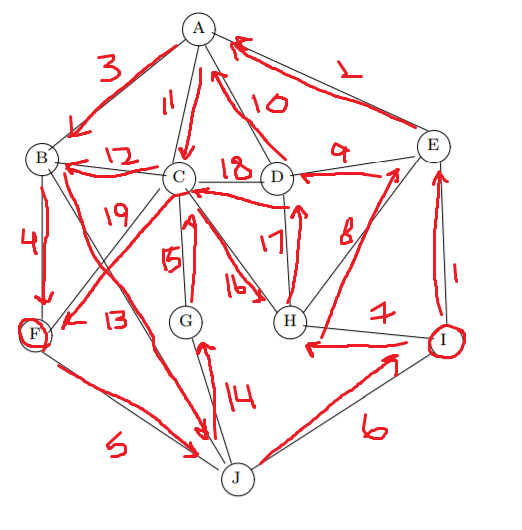
\includegraphics[height=150px]{hw3apa.png}

\underline{Problem B}

A directed graph is called strongly connected if there is a directed trail from any given node to
any other given node.

a. Prove that a directed graph that has a directd Euler Cycle must be strongly connected.

A directed graph with a directed Euler cycle must by definition traverse every edge. Starting at any point in the cycle, there is a path that traverses through every edge in the graph and therefore every connected vertex in the graph. This means that starting from any given vertex, a directed trail to any other given node can be formed by following the cycle.

b.  Is the converse true (meaning, if a directed graph is strongly connected, must it have a directed Euler
cycle)? If true, give a short proof. If false, show a counterexample.

It is not true.

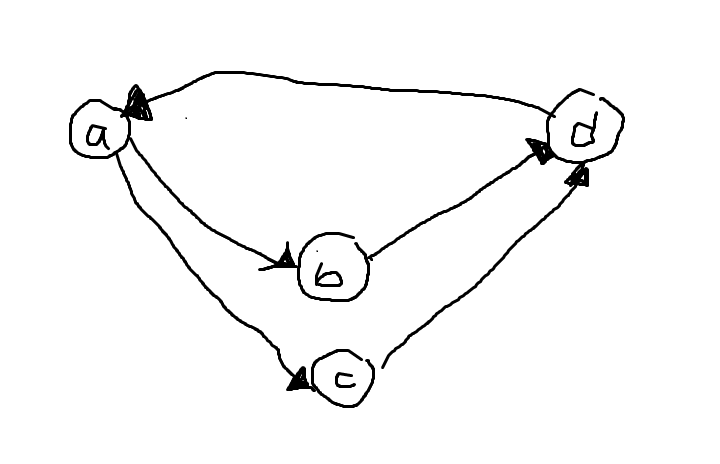
\includegraphics[height=150px]{hw3apb.png}

\end{document}
